\section{Requirements}
\label{sec:Requirements}

\subsection{Overview} 
The following section is on the requirements of the project and development methodology. 

\subsection{Development Methodology}
The stakeholders for this project is the project owner and sponsor, project advisor, and developer, Claire Mitchell, Elliot Forbes, and Austin Klum respectively. The end users are the students using the virtual reality tool for their learning and the instructors using the quiz management tool for assessment of student's comprehension of classroom material.
\\
The chosen development methodology for a project is an early and influential decision made that alters the course of development. As this was a solo-developer, web, and virtual reality project with a busy project sponsor, the decision was made to make use of an iterative agile methodology. An iterative agile approach focuses on delivering value to the product in fast small increments, rather than all at once. This approach allows software developers to adjust, refine, and review the development process to better provide value and output. This approach also allows for earlier risk identification and the flexibly to easily correct course.\\
\\
Traditional methodology follows the waterfall approach which \qquote{contains five phases of management, where each requires a deliverable from the previous phase to proceed}{waterfall}. The waterfall method is more suit for projects that follow a linear path and is fixed and rigid. The project did not have this rigidity or clarity of output, hence a more Agile approach was taken. The developer also made use of a KanBan board to help keep organized. 


\subsection{Course Creator}
This tool allows the project sponsor and verified users to create orienteering courses for the students to complete. Each course is comprised of locations which has a corresponding photo to accompany the location. To help with immersion and to best utilize the capabilities of virtual reality, the uploaded photos must be 360 Photos, also known as a photo sphere. This type of photo allows for the virtual reality tool to wrap the image around the user making a sphere, such that the user is able to look around as if they were really at that location. The tool also allows for locations to be added, updated, or deleted. Each location has a list of questions. There is no limit to the number of questions per location. The tool allows for each question to be added, updated, or deleted. Each question has a list of answers which can be of one to six possibilities. The tool allows for each answer to be added, updated, or deleted. \\
\\
Once a course has been completed by a student, a verified user can view the results from the course main dashboard. This dashboard lists the student ID, point score, time score, and total score. As security is important, the database is encrypted and requires an authorized administrator database account to access the data outside of the tool. \\
\\
For a user to be created, they must create an account with an email and password. Once the account is created, the user is immediately able to login, but will be unable to access any of the course creation or course results pages, limited only to the homepage and user settings. Each verified user has the capability to approve other users. In the user settings page, there exists a link to verify users. The verify users page list all users and their status of verified or not verified. From here a verified user can verify or un-verify other users by selecting the corresponding checkbox and saving. 


\subsubsection{Users}
Figure \ref{Course Creator Use Case Diagram} explains the use case diagram.

\begin{figure}[htb]
	\centering
	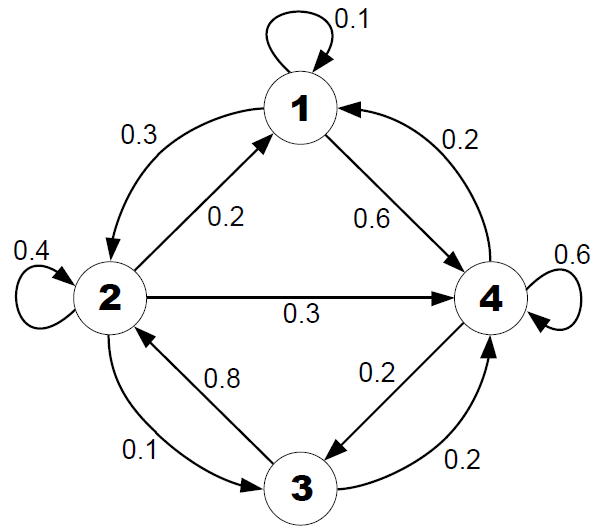
\includegraphics[width=.5\textwidth]{Requirements/assets/course-use-case-diagram.png}
	\caption[Course Creator Use Case Diagram]{\label{Course Creator Use Case Diagram}Course Creator Use Case Diagram}
\end{figure}

\subsubsection{Create Course Flow}
This section will include photos and written steps on how to use the course creator. 

\subsection{Virtual Reality Orienteering}
This tool is used by the students to complete the created orienteering courses that the project sponsor or verified user(s) created. Upon starting the program the user is prompted to enter their student ID using a "mallet" and tap virtual keyboard. Once the student has entered their student ID, they then select the course via a select list with a point and trigger arrow pointers buttons. After hitting the start button the student begins the course. The first location is loaded up and the student can look around the location. Upon touching the touch pad the first question and corresponding possible answers appears in the world view. As part of the orienteering spirit each question must be answered correctly to continue on to the next question. When a student answers incorrectly the button turns red and is disabled. When answered correctly the button flashes green and the next question and corresponding possible answers load. The student is graded on how quickly they came to the correct answer and, with the orienteering aspect in mind, the time to completely answer all the questions in a location. Each question is worth one point and each location time is worth one point. The score point is awarded divided by the number of attempts. This means that a question with four possible answers the following outcomes are possible: answered correctly has one point awarded, one incorrect attempt has .75 points awarded, two incorrect attempts has .5 points awarded, and three incorrect attempts has .25 points awarded. For the time aspect of the grade, the student has 100 seconds to complete the location, where each second is worth .01 points. This means if the student took 30 seconds to answer the questions and complete the location, they are awarded with .70 points. A time of 45 seconds is awarded .65 points. \\
\\
Upon answering all the questions for a location, the next location is loaded and the timer is reset. Once all locations have been completed a game over screen appears stating the student's point score, time score, total score, and what the maximum points awarded could be. 
\subsubsection{Users}
Figure \ref{Virutal Reality Orienteering Use Case Diagram} explains the use case diagram.

\begin{figure}[htb]
	\centering
	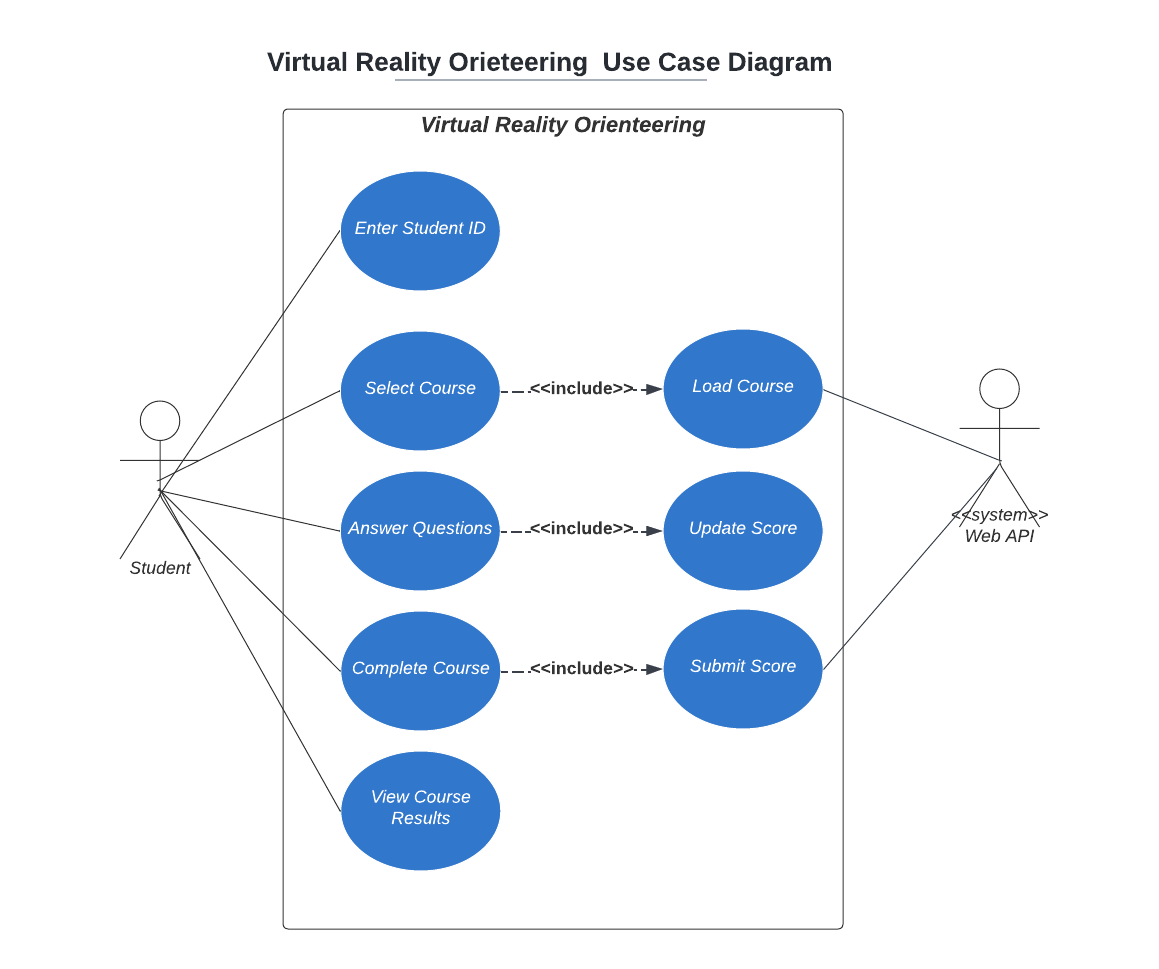
\includegraphics[width=.5\textwidth]{Requirements/assets/vr-use-case-diagram.png}
	\caption[Virutal Reality Orienteering Use Case Diagram]{\label{Virutal Reality Orienteering Use Case Diagram}Virtual Reality Orienteering Use Case Diagram}
\end{figure}

\subsubsection{Virtual Reality Orienteering Flow}
This section will include photos and written steps on the experience of the student completing a course.